\documentclass[12pt]{article}

%%%%%%%%%%%%%%%%%%%%%%%%%%%%%%%%%%%%%%%%%%%%%%%%%%%%%%%%%%%%%%%%%%%%%%%%%%%%%%%%
%                           Package preset for homework
%%%%%%%%%%%%%%%%%%%%%%%%%%%%%%%%%%%%%%%%%%%%%%%%%%%%%%%%%%%%%%%%%%%%%%%%%%%%%%%%
% Miscellaneous
\usepackage[margin=1in]{geometry}
\usepackage[utf8]{inputenc}
\usepackage{indentfirst}
\usepackage{blindtext}
\usepackage{graphicx}
\usepackage{xr-hyper}
\usepackage{hyperref}
\usepackage{enumitem}
\usepackage{color}
\usepackage{float}
% Math
\usepackage{latexsym}
\usepackage{amsfonts}
\usepackage{amssymb}
\usepackage{amsmath}
\usepackage{commath}
\usepackage{amsthm}
\usepackage{bbold}
\usepackage{bm}
% Physics
\usepackage{physics}
\usepackage{siunitx}
% Code typesetting
\usepackage{listings}
% Citation
\usepackage[authoryear]{natbib}
\usepackage{appendix}
\usepackage[capitalize]{cleveref}
% Title & name
\title{Homework}
\author{Tien Vo}
\date{\today}


%%%%%%%%%%%%%%%%%%%%%%%%%%%%%%%%%%%%%%%%%%%%%%%%%%%%%%%%%%%%%%%%%%%%%%%%%%%%%%%%
%                   User-defined commands and environments
%%%%%%%%%%%%%%%%%%%%%%%%%%%%%%%%%%%%%%%%%%%%%%%%%%%%%%%%%%%%%%%%%%%%%%%%%%%%%%%%
%%% Misc
\sisetup{load-configurations=abbreviations}
\newcommand{\due}[1]{\date{Due: #1}}
\newcommand{\hint}{\textit{Hint}}
\let\oldt\t
\renewcommand{\t}[1]{\text{#1}}

%%% Bold sets & abbrv
\newcommand{\N}{\mathbb{N}}
\newcommand{\Z}{\mathbb{Z}}
\newcommand{\R}{\mathbb{R}}
\newcommand{\Q}{\mathbb{Q}}
\let\oldP\P
\renewcommand{\P}{\mathbb{P}}
\newcommand{\LL}{\mathcal{L}}
\newcommand{\FF}{\mathcal{F}}
\newcommand{\HH}{\mathcal{H}}
\newcommand{\NN}{\mathcal{N}}
\newcommand{\ZZ}{\mathcal{Z}}
\newcommand{\RN}[1]{\textup{\uppercase\expandafter{\romannumeral#1}}}
\newcommand{\ua}{\uparrow}
\newcommand{\da}{\downarrow}

%%% Unit vectors
\newcommand{\xhat}{\vb{\hat{x}}}
\newcommand{\yhat}{\vb{\hat{y}}}
\newcommand{\zhat}{\vb{\hat{z}}}
\newcommand{\nhat}{\vb{\hat{n}}}
\newcommand{\rhat}{\vb{\hat{r}}}
\newcommand{\phihat}{\bm{\hat{\phi}}}
\newcommand{\thetahat}{\bm{\hat{\theta}}}

%%% Other math stuff
\providecommand{\units}[1]{\,\ensuremath{\mathrm{#1}}\xspace}
% Set new style for problem
\newtheoremstyle{problemstyle}  % <name>
        {10pt}                   % <space above>
        {10pt}                   % <space below>
        {\normalfont}           % <body font>
        {}                      % <indent amount}
        {\bfseries\itshape}     % <theorem head font>
        {\normalfont\bfseries:} % <punctuation after theorem head>
        {.5em}                  % <space after theorem head>
        {}                      % <theorem head spec (can be left empty, 
                                % meaning `normal')>

% Set problem environment
\theoremstyle{problemstyle}
\newtheorem{problemenv}{Problem}[section]
\newenvironment{problem}[1]{%
  \renewcommand\theproblemenv{#1}%
  \problemenv
}{\endproblemenv}
% Set lemma environment
\newenvironment{lemma}[2][Lemma]{\begin{trivlist}
\item[\hskip \labelsep {\bfseries #1}\hskip \labelsep {\bfseries #2.}]}{\end{trivlist}}
% Set solution environment
\newenvironment{solution}{
    \begin{proof}[Solution]$ $\par\nobreak\ignorespaces
}{\end{proof}}
\numberwithin{equation}{problemenv}

%%% Page format
\setlength{\parindent}{0.5cm}
\setlength{\oddsidemargin}{0in}
\setlength{\textwidth}{6.5in}
\setlength{\textheight}{8.8in}
\setlength{\topmargin}{0in}
\setlength{\headheight}{18pt}

%%% Code environments
\definecolor{dkgreen}{rgb}{0,0.6,0}
\definecolor{gray}{rgb}{0.5,0.5,0.5}
\definecolor{mauve}{rgb}{0.58,0,0.82}
\lstset{frame=tb,
  language=Python,
  aboveskip=3mm,
  belowskip=3mm,
  showstringspaces=false,
  columns=flexible,
  basicstyle={\small\ttfamily},
  numbers=none,
  numberstyle=\tiny\color{gray},
  keywordstyle=\color{blue},
  commentstyle=\color{dkgreen},
  stringstyle=\color{mauve},
  breaklines=true,
  breakatwhitespace=true,
  tabsize=4
}
\lstset{
  language=Mathematica,
  numbers=left,
  numberstyle=\tiny\color{gray},
  numbersep=5pt,
  breaklines=true,
  captionpos={t},
  frame={lines},
  rulecolor=\color{black},
  framerule=0.5pt,
  columns=flexible,
  tabsize=2
}


\title{Homework 3: Phys 7230 (Spring 2022)}
\due{February 21, 2022}

\begin{document}
\maketitle
%%%%%%%%%%%%%%%%%%%%%%%%%%%%%%%%%%%%%%%%%%%%%%%%%%%%%%%%%%%%%%%%%%%%%%%%%%%%%%%
\begin{problem}{1}[Derivation of ensembles]~\\
(a) Grand canonical ensemble~\\
Start with the expression
\begin{equation}
    W\qty[\qty{n_q}]=\frac{\mathcal{N}!}{\prod_qn_q!} 
\end{equation}
for the number of configurations in a grandcanonical ensemble consisting of
$\mathcal{N}$ systems with a set $\qty{n_q}$ describing the number of systems
with energy $E_q$ and number of particles $N_q$, discussed in lectures.
Utilizing lowest order Stirling approximation, maximize $W\qty[\qty{n_q}]$ over
$n_q$, subject to three constraints,
\begin{equation}
    \sum_qn_q=\NN,\qquad\sum_qn_qE_q=E\NN,\qquad\sum_qn_qN_q=N\NN ,
\end{equation}
imposed via Lagrange multiplier $\gamma,\beta,\alpha,$ with $E$ and $N$ the
average energy and particle number in the ensemble, derive the most likely
$n_q^\ast$ and thereby obtain the grandcanonical probability distribution
$P_q=n_q^\ast/\NN$.

\textit{Hint}: Maximizing $\ln W$ may be more convenient.
\begin{solution}
First, using Stirling approximation, we write
\begin{equation}
    \ln W=\NN\ln\NN -\NN-\sum_q\qty(n_q\ln n_q - n_q)
    =\NN\ln\NN-\sum_qn_q\ln n_q.
\end{equation}
Extremizing this function, we calculate
\begin{align}
    \grad(\ln W)
    &-\gamma\grad\qty(\sum_qn_q-\NN)
    -\beta\grad\qty(\sum_qn_qE_q-E\NN)
    -\alpha\grad\qty(\sum_qn_qN_q-N\NN)\notag\\
    \qquad&=
    \qty[\ln\NN-1-\ln n_q+1+\beta(E-E_q)+\alpha(N-N_q)]\hat{e}_q=0.
\end{align}
where $\grad=(\partial/\partial n_q)\hat{e}_q$ (Einstein summation used
implicitly). Inverting each expression, we get
\begin{equation}\label{p1a:n_q}
    \frac{n_q}{\NN}=e^{\beta(E-E_q)+\alpha(N-N_q)}.
\end{equation}
By the normalization condition,
\begin{equation}
    1=\sum_q\frac{n_q}{\NN}=e^{\beta E+\alpha N}\sum_qe^{-\beta E_q-\alpha N_q}
    =e^{\beta E+\alpha N}\ZZ.
\end{equation}
where $\beta=1/k_BT$ and $\alpha=-\mu\beta$. Then, letting $n_q=n_q^\ast$, the
most probable state satisfying \eqref{p1a:n_q}, we can write the probability
distribution as
\begin{equation}
    P_q=\frac{n_q^\ast}{\NN}=\frac{e^{-\beta E_q-\alpha N_q}}\ZZ  .
\end{equation}
\end{solution}
%%%%%%   

(b) Derivation redux

Let us rederive all three ensembles distributions in a more streamlined way by
focusing on $P_q$ and noting that $P_q$ can be determined by maximizing the
(Shannon's) entropy $S=-k_B\sum_qP_q\ln P_q$ subject to the appropriate number
of constraints for each ensemble. Thus, derive

\qquad(i) Microcanonical ensemble subject to its one constraint, showing that it
is just given by a normalized \textit{constant} $P_q=1/\Omega$.

\qquad(ii) Canonical ensemble subject to its two constraints, showing that it 
is given by the Gibbs form.

\qquad(iii) Grandcanonical ensemble subject to its three constraints, showing
that it is given by the Gibbs form.
\begin{solution}
\qquad(i) The constraint for the microcanonical ensemble is the normalization
condition
\begin{equation}\label{p1b:normalization_condition}
    \sum_qP_q=1 .
\end{equation}
Then, we differentiate to find $P_q$ that extremizes $S$
\begin{equation}
   \grad(S)-\lambda\grad\qty(\sum_qP_q-1)
   =\qty[-k_B\qty(\ln P_q+1)-\lambda_1]\hat{e}_q
   \Rightarrow P_q=e^{-1-\lambda/k_B}.
\end{equation}
Plugging this back into the normalization condition, we get
\begin{equation}
    \sum_qP_q=e^{-1-\lambda_1/k_B}\sum_q1
    =e^{-1-\lambda_1/k_B}\Omega,
\end{equation}
where $\Omega=\sum_\qty{q_i}1$ is the multiplicity of the system. Then we can
rewrite the probability distribution function
\begin{equation}
    P_q=\frac1\Omega, 
\end{equation}
which is a constant, indicating a uniform distribution. Also, we can invert to
solve for $\lambda_1$
\begin{equation}
    \lambda_1=S_t-k_B, 
\end{equation}
where $S_t=k_B\ln\Omega$ is the thermodynamic entropy.

\qquad(ii) In addition to the normalization condition
\eqref{p1b:normalization_condition}, we add a constraint
\begin{equation}
    \sum_qE_qP_q=E, 
\end{equation}
where $E$ is the average energy of the system. Then, the $P_q$ that extremizes
$S$ satisfies
\begin{equation}
    \qty[-k_B\qty(\ln P_q+1)-\lambda_1-\lambda_2E_q]\hat{e}_q=0
    \Rightarrow P_q=e^{-1-\lambda_1/k_B-\lambda_2E_q/k_B}.
\end{equation}
Applying the normalization,
\begin{equation}
    1=\sum_qP_q=e^{-1-\lambda_1/k_B}\sum_qe^{-\lambda_2E_q/k_B}
    = e^{-1-\lambda_1/k_B}\sum_qe^{-\beta E_q}
    \Rightarrow e^{-1-\lambda_1/k_B}=\frac1{Z},
\end{equation}
where we have let the constant $\lambda_2=1/T$, with $T$ the equilibrium
temperature, and $Z$ is the partition function of the canonical ensemble. It
then follows that the distribution function
\begin{equation}
    P_q=\frac{e^{-\beta E_q}}{Z} 
\end{equation}
has the Gibbs form.

(iii) The third constraint to add is
\begin{equation}
    \sum_qN_qP_q=N,
\end{equation}
where $N$ is the average number of particles per partition. Then $P_q$
extremizing $S$ satisfies
\begin{equation}
    -k_B\qty(\ln P_q+1)-\lambda_1-\lambda_2E_q-\lambda_3N_q
    =-k_B\ln P_q-S_t-E_q/T-\lambda_3 N_q=0,
\end{equation}
where we have replaced the first two Lagrange multipliers with physical
quantities derived in (i-ii). The probability distribution function is
\begin{equation}
    P_q=e^{-S-\beta E_q-\lambda_3N_q/k_B}=e^{-S-\beta E_q+\beta\mu N_q},
\end{equation}
where we have let the constant $\lambda_3=-\mu/T$. Then, with the normalization
condition,
\begin{equation}
    1=e^{-S}\sum_qe^{-\beta(E_q+\mu N_q)}=e^{-S}\ZZ, 
\end{equation}
and the probability distribution function can be written as
\begin{equation}
    P_q=\frac{e^{-\beta(E_q+\mu N_q)}}{\ZZ}, 
\end{equation}
which has the Gibbs form.
\end{solution}

%%%%%%   

(c) Recall the expression for $\Omega(E)$ for the microcanonical ensemble of a
3d ideal Boltzmann gas of $N$ particles. Using it, calculate the probability
$P_\epsilon$ of a \textit{particular} particle to have energy in the
neighborhood of $\epsilon\ll E$.

From your answer for $P_\epsilon$ and comparing it with the standard
Boltzmann-Gibbs weight, read off the corresponding effective temperature of this
single particle in terms of $E$ and $N$.

\textit{Hint}: (i) From above total $\Omega(E)$ first think about the number of
states (sub-multiplicity) $\Omega_\epsilon(E)$ for one of the particle to have
energy $\epsilon$ and the remaining $N-1$ sharing the remaining energy. (ii)
Note that $P_\epsilon=\Omega_\epsilon/\Omega$. (iii) Use Stirling's
approximation and $\epsilon\ll E$ to simplify your answer.

\begin{solution}
From Sackur-Tetrode, we can write the multiplicity as $\Omega=e^{S/k_B}
=(V^N/N!)f(N,E)$ where
\begin{equation}
    f(N,E)=e^{5N/2}\qty(\frac{4\pi mE}{3Nh^2})^{3N/2}.
\end{equation}
Then, we note that there is only one way to distribute an energy of $\epsilon$
into a particular particle. Thus, the multiplicity for the entire system of one
particle of energy $\epsilon$ and $N-1$ particles of energy $E-\epsilon$ is
\begin{align}
    \Omega_\epsilon
    &=\frac{V^{N-1}}{(N-1)!}f(N-1,E-\epsilon)\notag\\
    &=\frac{V^{N-1}}{(N-1)!}e^{5(N-1)/2}\qty(\frac{4\pi
    m(E-\epsilon)}{3(N-1)h^2})^{3(N-1)/2}\notag\\
    &\approx\frac{V^{N-1}}{(N-1)!}e^{5(N-1)/2}\qty(\frac{4\pi
    m(E-\epsilon)}{3Nh^2})^{3(N-1)/2}.
\end{align}
The probability is thus
\begin{align}
    P_\epsilon
    &=\frac{\Omega_\epsilon}{\Omega}\notag\\
    &\approx\frac{N}{V}e^{-5/2}\qty(\frac{4\pi m E}{3Nh^2})^{-3/2}
        \qty(1-\frac{\epsilon}{E})^{3(N-1)/2}\notag\\
    &\approx\frac{N}{V}e^{-5/2}\qty(\frac{4\pi m E}{3Nh^2})^{-3/2}
        e^{-3(N-1)\epsilon/2E},
\end{align}
which follows the Gibbs form if the effective temperature is defined as
\begin{equation}
    k_BT_\text{eff}=\frac{2E}{3(N-1)}.
\end{equation}
\end{solution}

%%%%%%   

(d) Variance (i.e., mean-squared fluctuations) in the number of particles $N$ in
the grand canonical ensemble is given by $\expval{(\Delta N)^2}$. Show that
quite generally it is given by
\begin{equation}
    N_\text{rms}^2=\expval{\qty(\Delta
    N)^2}=-\eval{\frac{\partial\overline{N}}{\partial\alpha}}_{\beta,V}
    =\eval{\frac{\partial^2(\ln\mathcal{Z})}{\partial\alpha^2}}_{\beta,V}
\end{equation}
\begin{solution}
First, from $\ZZ$, we can calculate
\begin{align}\label{p1d:dZda}
    \frac{\partial\ZZ}{\partial\alpha}
    =\frac{\partial}{\partial\alpha}\sum_qe^{-\beta E_q-\alpha N_q}
    =-\sum_qN_qe^{-\beta E_q-\alpha N_q}
    =-\expval{N}\ZZ,
\end{align}
and
\begin{align}
    \frac{\partial^2\ZZ}{\partial\alpha^2}
    =\sum_qN_q^2e^{-\beta E_q-\alpha N_q}
    =\expval{N^2}\ZZ.
\end{align}
Differentiating \eqref{p1d:dZda} again, we get
\begin{equation}
    \expval{N^2}\ZZ=-\frac{\partial\expval{N}}{\partial\alpha}\ZZ
    +\expval{N}^2\ZZ
    \Rightarrow\expval{(\Delta
    N)^2}=\expval{N^2}-\expval{N}^2=-\frac{\partial\expval{N}}{\partial\alpha}.
\end{equation}
Also,
\begin{equation}
    \frac{\partial(\ln\ZZ)}{\partial\alpha}=-\expval{N}.
\end{equation}
So taking the differentation again leads us to the second equality
\begin{equation}
    \frac{\partial^2(\ln\ZZ)}{\partial\alpha^2}=-\frac{\partial\expval{N}}{\partial\alpha}
    .
\end{equation}
\end{solution}
\end{problem}
\newpage
%%%%%%%%%%%%%%%%%%%%%%%%%%%%%%%%%%%%%%%%%%%%%%%%%%%%%%%%%%%%%%%%%%%%%%%%%%%%%%%   
%%%%%%%%%%%%%%%%%%%%%%%%%%%%%%%%%%%%%%%%%%%%%%%%%%%%%%%%%%%%%%%%%%%%%%%%%%%%%%%
\begin{problem}{2}[Ultra-relativistic gas]
Consider a non-interacting 3d gas of identical ultra-relativistic particles
(i.e., ignoring their mass), with a dispersion $\epsilon_i=p_ic$, at temperature
$T$ and chemical potential $\mu$, where
$p_i=\abs{\vb{p}_i}=\sqrt{p_{xi}^2+p_{yi}^2+p_{zi}^2}$.

Following similar steps that we did in class for nonrelativistic Boltzmann gas,
compute:

(a) Grandcanonical partition function, $\ZZ(\mu,T)$ by first computing the
canonical one, $Z(N,T)$, introducing fugacity and then summing over $N$.

\textit{Hint}: it is nice to do the integral in the spherical coordinate system.
\begin{solution}
By definition, the canonical partition function is
\begin{align}
    Z(N,T)
    &=\frac1{N!}\prod_{i=1}^N\qty[\int\frac{d^3\vb{r}_id^3\vb{p}_i}{(2\pi\hbar)^3}]e^{-\beta\sum_{j=1}^N\epsilon_i}\notag\\
    &=\frac{V^N}{N!}\frac{1}{h^{3N}}\prod_{i=1}^N\qty[\int
    d^3\vb{p}_i\exp\qty(-\beta\abs{\vb{p}_i}c)]\notag\\
    &=\frac{V^N}{N!}\frac1{h^{3N}}\qty[\int_0^{4\pi}d\Omega\int_0^\infty dp
p^2e^{-\beta pc}]^N\notag\\
    &=\frac{V^N}{N!}\qty[\frac{4\pi}{\qty(\beta hc)^3}]^N
        \qty[\int_0^\infty dxx^2e^{-x}]^N\tag{$x=\beta pc$}\\
    &=\frac1{N!}\qty[\frac{8\pi V}{(\beta hc)^3}]^N.
\end{align}
The grandcanonical partition function is then
\begin{align}\label{p2a:Zb}
    \ZZ(\alpha,\beta)=\sum_{N=0}^\infty z^NZ(N,T)
    =\sum_{N=0}^\infty\frac1{N!}\qty[\frac{8\pi zV}{(\beta hc)^3}]^N
    =\exp\qty[\frac{8\pi zV}{(\beta hc)^3}]
    =\exp\qty[\frac{8\pi V}{(\beta hc)^3}e^{-\alpha}],
\end{align}
where $z=e^{-\alpha}$ is the fugacity. Unpacking these definitions, we get
\begin{equation}\label{p2a:Z}
    \ZZ(\mu,T)=\exp\qty[8\pi Ve^{\mu/k_BT}\qty(\frac{k_BT}{hc})^3].
\end{equation}
\end{solution}

%%%%%%%%%%%
(b) Grandcanonical free energy $\FF(\mu,T)$.
\begin{solution}
From \eqref{p2a:Z}, it is a straightforward calculation to get
\begin{equation}
    \FF(\mu,T)=-k_BT\ln\ZZ
    =-8\pi Vk_BT\qty(\frac{k_BT}{hc})^3e^{\mu/k_BT}.
\end{equation}
\end{solution}

%%%%%%%%%%%
(c) Average energy $E(\mu,T)$.
\begin{solution}
Using the expression of $\ZZ$ in terms of $\alpha$ and $\beta$ \eqref{p2a:Zb}, 
we can calculate
\begin{align}\label{p2c:E}
    E(\mu,T)
    &=-\frac{\partial(\ln\ZZ)}{\partial\beta}\notag\\
    &=-\frac{\partial}{\partial\beta}\qty[\frac{8\pi V}{(\beta
    hc)^3}e^{-\alpha}]\notag\\
    &=\frac1\beta\frac{24\pi V}{(\beta hc)^3}e^{-\alpha}\notag\\
    &=24\pi Vk_BT\qty(\frac{k_BT}{hc})^3e^{\mu/k_BT}.
\end{align}
\end{solution}

%%%%%%%%%%%
(d) Average particle number $N(\mu,T)$.
\begin{solution}
Recall that $z=e^{\alpha}$, we can calculate
\begin{align}
    N(\mu,T)
    =-\frac{\partial}{\partial\alpha}\qty[\frac{8\pi V}{(\beta
    hc)^3}e^{-\alpha}]
    =8\pi V\qty(\frac{k_BT}{hc})^3e^{\mu/k_BT}
    =\frac{E}{3k_BT}.
\end{align}
\end{solution}

%%%%%%%%%%%
(e) Pressure $P(\mu,T)$. Find the relation between $P$ and $E$.
\begin{solution}
By definition, we write
\begin{align}
    P(\mu,T)
    =\frac1\beta\frac{\partial(\ln\ZZ)}{\partial V}
    =8\pi k_BT\qty(\frac{k_BT}{hc})^3e^{\mu/k_BT}
    =\frac{Nk_BT}{V}.
\end{align}
Together with \eqref{p2c:E}, we can write
\begin{equation}
    E=3PV.
\end{equation}
\end{solution}

%%%%%%%%%%%
(f) Heat capacities $C_v$ and $C_p$ and find the ratio $\gamma=C_p/C_v$.

\textit{Hint}: While in thermodynamics observables are obtained by appropriate
derivative of the free energy $\FF$, in statistical mechanics, it is often
mathematically more convenient (but equivalent) to instead differentiate
$q=\ln\ZZ$.
\begin{solution}
By definition,
\begin{align}
    C_v=\frac{\partial E}{\partial T}=3Nk_B,
    \qquad\t{and}\qquad
    C_p=C_v+P\frac{\partial V}{\partial T}
    =3Nk_B+Nk_B=4Nk_B.
\end{align}
Thus, $\gamma=C_p/C_v=4/3$.
\end{solution}
\end{problem}
\newpage
%%%%%%%%%%%%%%%%%%%%%%%%%%%%%%%%%%%%%%%%%%%%%%%%%%%%%%%%%%%%%%%%%%%%%%%%%%%%%%%
%%%%%%%%%%%%%%%%%%%%%%%%%%%%%%%%%%%%%%%%%%%%%%%%%%%%%%%%%%%%%%%%%%%%%%%%%%%%%%%
\begin{problem}{3}[Boltzmann diatomic gas]
Consider a noninteracting 3d gas of $N$ nonrelativistic \textit{diatomic}
molecules, e.g., $O_2$, at temperature $T$, in a box of volume $V$, as dicussed
in lecture and described by a Hamiltonian,
\begin{equation}
    \HH=\frac{\vb{p}_1^2}{2m}+\frac{\vb{p}_2^2}{2m}+U\qty(\abs{\vb{r}_1-\vb{r}_2})
    ,
\end{equation}
where the potential has a minimum at a nonzero value of the average bond length
$l$, with
\begin{equation}
    U(\abs{\vb{r}})=\frac12m\omega_0^2\qty(r-l)^2=\frac12m\omega_0^2\qty(\sqrt{x^2+y^2+z^2}-l)^2.
\end{equation}
Let's calculate the thermodynamics of this gas by computing the canonical
partition function,
\begin{equation}
    Z(T,V,N)=\frac1{N!}\prod_i^N\qty[\int\frac{d^3\vb{r}_{1i}d^3\vb{p}_{1i}d^3\vb{r}_{2i}d^3\vb{p}_{2i}}{(2\pi\hbar)^{6}}]e^{-\beta\HH\qty[\qty{\vb{p}_{1i},\vb{p}_{2i},\vb{r}_{1i},\vb{r}_{2i}}]},
\end{equation}
where $\vb{r}_{1i},\vb{r}_{2i}$, and $\vb{p}_{1i},\vb{p}_{2i}$ are position and
momentum of, respectively, atom 1 and 2 in a molecule $i$.

Although this looks complicated by now, we know that for noninteracting
molecules we have a simplification with partition function reducing to that of a
single molecule according to $Z(T,V,N)=Z(T,V,1)^N/N!$. So let's focus on the
computation of $Z(T,V,1)$.

(a) Compute $Z(T,V,1)$ and obtain from it (i) free energy $F(T,V,1)$, and (ii)
heat capacity $c_v(T)$ per molecule, and plot the latter as a function of $T$.

\textit{Hint}: (i) As discussed in class the center of mass momentum $\vb{P}$
and position $\vb{R}$ will decouple giving their own multipicative contribution
to $Z(T,V,1)$. (ii) The relative momentum $\vb{p}$ will also decouple, so the
nontrivial part of the problem reduces to the trace over the relative coordinate
$\vb{r}$, i.e., to a \textit{three}-dimensional integral $\int d^3\vb{r}$. Note
however, that given the form of $U(\abs{\vb{r}})$ above, this last integral is
not a standard Gaussian. To solve the problem express the above physical
observables $F(T,V,1)$ and $c_v(T)$ in terms of this last integral over
$\vb{r}$ (that can still be simplified to a single one-dimensional integral,
utilizing rotational invariance). Then compute the final integral numerically
for a given value of bond length $l$ and plot the corresponding $c_v(T)$. Make
sure to demonstrate, not just accept all of the above ``hint'' steps.
\begin{solution}
See part (b).
\end{solution}

%%%%%%%%%%
(b) Identify the low and high temperature asymptotic number of degrees of
freedom, $n_\text{dof}$ per molecule, appearing through the heat capacity plot
vs. $T$, and thereby confirming our in class discussion.
\begin{solution}
By definition, the canonical partition function for a single molecule is
\begin{align}\label{p3a:Z1_1}
    Z_1
    &=\frac1{(2\pi\hbar)^6}\int d^3\vb{r}_1d^3\vb{p}_1 d^3\vb{r}_2d^3\vb{p}_2
    \exp\qty[-\frac12\frac{\beta}{m}(\vb{p}_1^2+\vb{p}_2^2)-\beta U(r)]\notag\\
    &=\frac1{(2\pi\hbar)^6}\qty(\int_{-\infty}^\infty dp e^{-\beta p^2/2m})^6
    \int d^3\vb{r}_1d^3\vb{r}_2e^{-\beta U(r)}\notag\\
    &=\frac1{(2\pi)^3\hbar^6}\qty(\frac{m}{\beta})^3
    \int d^3\vb{r}_1d^3\vb{r}_2e^{-\beta U(r)}.
\end{align}
Now, we define the transformation $T:\R^6\mapsto\R^6$ as follows
\begin{equation}
    T(\vb{r}_1,\vb{r}_2)
    =\mqty[\vb{r}_1-\vb{r}_2&(1/2)\qty(\vb{r}_1+\vb{r}_2)]^T .
\end{equation}
The Jacobian of $T$ is
\begin{equation}
    \norm{\grad{T}}
    =\det\mqty(\mathbb{1}_3&(1/2)\mathbb{1}_3\\-\mathbb{1}_3&(1/2)\mathbb{1}_3)
    =1,
\end{equation}
where $\mathbb{1}_3$ is the 3x3 identity matrix. Thus, the integration in
\eqref{p3a:Z1_1} becomes
\begin{align}\label{p3a:Int}
    \int d^3\vb{r}_1d^3\vb{r}_2e^{-\beta U(r)}
    =\int d^3\vb{r}d^3\vb{R}\norm{\grad{T}}e^{-\beta U(r)}
    =4\pi V_R\int_0^\infty dr r^2\exp\qty[-\frac12\beta m\omega_0^2(r-l)^2]
\end{align}
where we have let $V_R=\int d^3\vb{R}$, which blows up. However, since the free
energy is $F\sim\ln Z_1\sim\ln V_R+\t{other terms}$, we can later redefine the 
ground energy at $F_0\approx\ln V_R$ to get out of this situation, which is
physically valid. Now, set $\beta_\ast=1/m\omega_0^2l^2=1/k_BT_\ast$ and
$u=(r/l)\sqrt{\beta/\beta_\ast}$, we can rewrite the integral \eqref{p3a:Int} as
\begin{align*}
    4\pi V_Rl^3\qty(\frac{\beta_\ast}{\beta})^{3/2} I_1(x),
\end{align*}
where we have defined
\begin{equation}
    I_1(x)\equiv\int_0^\infty duu^2e^{-(u-\sqrt{x})^2/2}.
\end{equation}
The partition function is now
\begin{align}
    Z_1
    =\frac1{2\pi^2}\frac{V_R}{l^3}\frac1{(\hbar\omega_0)^6}\frac1{\beta_\ast^{3/2}\beta^{9/2}}I_1(\beta/\beta_\ast).
\end{align}

It then follows that (i) the free energy is
\begin{equation}
    F=-k_BT\ln Z_1 
    =-k_BT\ln\qty[\frac{V_R/l^3}{2\pi^2(\beta_\ast\hbar\omega_0)^6}]
    -k_BT\ln\qty[\qty(\frac{\beta_\ast}{\beta})^{9/2}I_1(\beta/\beta_\ast)],
\end{equation}
where the first term may be set to be the temperature-dependent ground energy.
The heat capacity is
\begin{align}\label{p3b:Cv}
    c_v
    &=\frac{\partial E}{\partial T}\notag\\
    &=k_B\beta^2\frac{\partial^2(\ln Z_1)}{\partial\beta^2}\notag\\
    &=\frac92k_B+k_B\beta^2\frac{I_1(x)I_1''(x)-\qty[I_1'(x)]^2}
        {\qty[I_1(x)]^2}\notag\\
    &=\frac92k_B+k_B\frac{I_1(x)I_3(x)-I_2(x)}{\qty[I_1(x)]^2},
\end{align}
where the argument of the $I_i$ functions are $x=\beta/\beta_\ast=T_\ast/T$, and
we have used Mathematica to solve the integrals $I_1,I_2,I_3$ numerically as
follows
\begin{subequations}
    \begin{align}
        I_1(x)&=-2I_3(x)+\sqrt{\frac\pi2}\qty(1+x)
            \qty[1+\erf\qty(\sqrt{\frac{x}{2}})]\label{p3b:I1}\\
        I_2(x)=\frac{\partial
    I_1(x)}{\partial\beta}&=\qty{-2I_3(x)+\sqrt{\frac\pi2}x\qty[1+\erf\qty(\sqrt{\frac{x}{2}})]}^2\label{p3b:I2}\\
        I_3(x)=\frac{\partial^2 I_1(x)}{\partial\beta^2}
        &=-\frac12\sqrt{x}e^{-x/2}\label{p3b:I3},
    \end{align} 
\end{subequations}
where $\erf(x)$ is the well-known error function. A plot of \eqref{p3b:Cv} is
given in \cref{fig:p3a} with the crossover temperature
$T_\ast=1/k_B\beta_\ast=m\omega_0^2l^2/k_B$. We observe that at the high
temperature limit, $n_\text{dof}=2c_v/k_B\to9$ degrees of freedom, while
$n_\text{dof}\to7$ as $T\to0$, in agreement with the in-class discussion.
\begin{figure}[H]
    \centering
    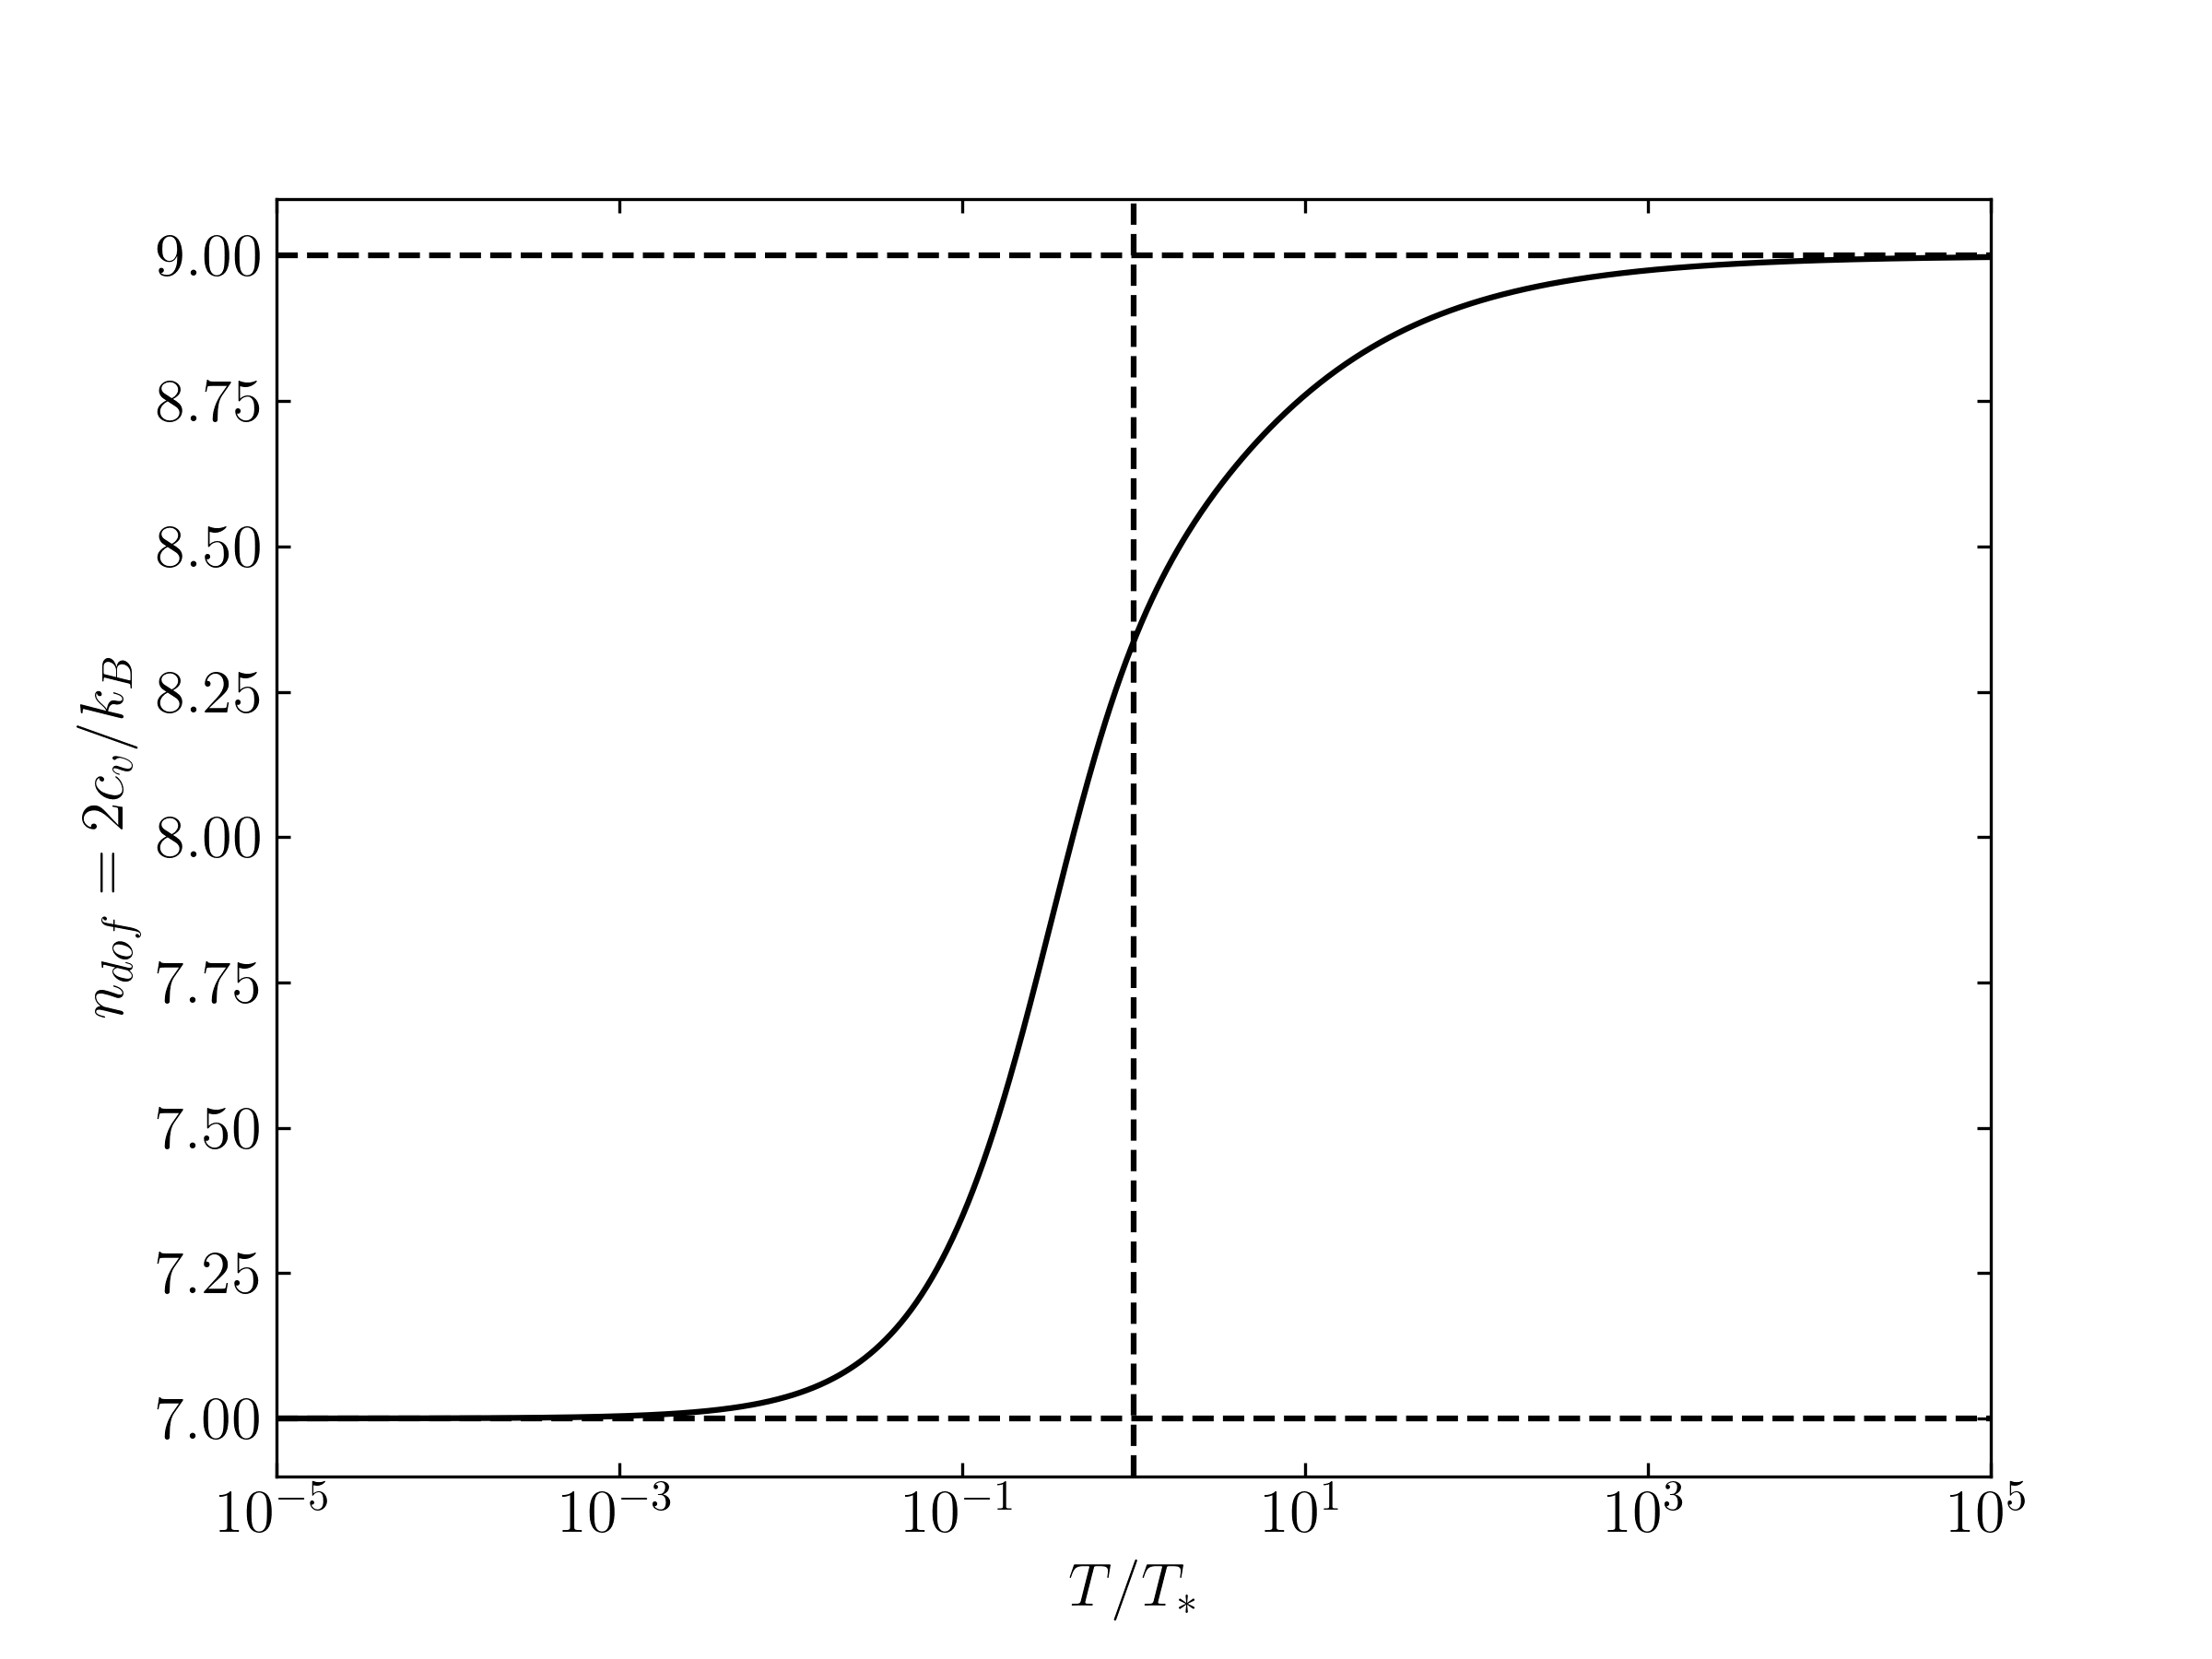
\includegraphics[width=0.8\textwidth]{p3a.png}
    \caption{Number of degrees of freedom per molecule in terms of
        temperature in a Boltzmann diatomic gas.}
        \label{fig:p3a}
\end{figure}
\end{solution}

%%%%%%%%%%
(c) By examining your analytical expression (before doing the final numerical
integral over $r$ above), give a dimensionless parameter in terms of
$l,T,\hdots$ that determines $T_\ast$ and controls whether one is in low $T\ll
T_\ast$ or high $T\gg T_\ast$ limits of $c_v(T)$. What is $T_\ast$?
\begin{solution}
First, note that $I_3\to0$ at both limits (low temperature -- $x\to\infty$,
and high temperature -- $x\to0$). Thus, the heat capacity at the extremes is
\begin{equation}
    \frac{c_v}{k_B}
    \approx\frac92-\frac{I_2(x)}{\qty[I_1(x)]^2}.
\end{equation}

Now, at high temperature ($T\gg T_\ast$ and $x\to0$), the error function
vanishes. Thus, $I_1\to\sqrt{\pi/2}$, while $I_2\to0$. So the heat capacity is
$c_v\approx (9/2)k_B$, as expected from \cref{fig:p3a}.

At low temperature ($x\to\infty$), the error function approaches unity. So $I_2$
grows as $2\pi x^2$, while $I_1^2$ grows as $2\pi(1+x)^2$. Both of them grows at
the same rate (quadratically), thus, by L'Hôpital's Rule,
\begin{equation}
    \frac{c_v}{k_B}=\frac92-\lim_{x\to\infty}\frac{x^2}{(1+x)^2} 
    =\frac92-1=\frac72,
\end{equation}
as expected!
\end{solution}

%%%%%%%%%%
(d) Now go back to the original Hamiltonian and in particular to the nontrivial
``difficult'' part involving the potential $U(\abs{\vb{r}})$ and neglect the
bond length $l$, setting it to 0. Using this simplification, recompute
$Z(T,V,1)$ (now best done in Cartesian coordinates using Gaussian integrals
calculus) and the corresponding heat capacity $c_v(T)$ per particle and compare
it with your above result for nonzero $l$, particularly with the high $T$ limit
of the plot.
\begin{solution}
For $l=0$, the canonical partition 
function is now
\begin{align}
Z&=\frac1{N!h^{6N}}\prod_{i=1}^N\qty[\int d^3\vb{r}_{1i} d^3\vb{p}_{1i}
d^3\vb{r}_{2i}d^3\vb{p}_{2i}\exp\qty[-\frac12\frac{\beta}{m}\qty(\vb{p}_{1i}^2+\vb{p}_{2i}^2)-\frac12\beta
m\omega_0^2r^2]]\notag\\
 &=\frac1{N!h^{6N}}\qty[\int_{-\infty}^\infty dp e^{-(1/2)(\beta/m)p^2}]^{6N}
 \qty[\int_{-\infty}^\infty dx e^{-(1/2)\beta m\omega_0^2x^2}]^{3N}\notag\\
 &=\frac1{N!}\qty(\frac1{h^2}\frac{2\pi
 m}{\beta}\sqrt{\frac{2\pi}{\beta m\omega_0^2}})^{3N}\notag\\
 &=\frac1{N!}\frac1{\hbar^{6N}}\qty(\frac{m}{2\pi\beta^3\omega_0^2})^{3N/2}.
\end{align}
Then, the free energy is
\begin{equation}
    F=-k_BT\ln Z
    =-k_BT\ln\qty[\frac1{N!}\frac1{\hbar^{6N}}\qty(\frac{m}{2\pi\omega_0^2})^{3N/2}]
    +\frac{9N}{2}k_BT\ln\beta.
\end{equation}
The first term grows linearly with $T$, so it vanishes under second-order
differentiation. Thus, the heat capacity is
\begin{equation}
    C_v=-T\frac{\partial^2F}{\partial T^2}
    =-\frac{9N}{2}T\frac{\partial^2}{\partial T^2}\qty(k_BT\ln\beta)
    =\frac{9Nk_B}{2}.
\end{equation}
So the heat capacity per molecule is $c_v=C_V/N=9k_B/2$, which indicates 9
degrees of freedom, in congruence with the high $T$ behavior in \cref{fig:p3a}.
\end{solution}
\end{problem}
\newpage
%%%%%%%%%%%%%%%%%%%%%%%%%%%%%%%%%%%%%%%%%%%%%%%%%%%%%%%%%%%%%%%%%%%%%%%%%%%%%%%

%%%%%%%%%%%%%%%%%%%%%%%%%%%%%%%%%%%%%%%%%%%%%%%%%%%%%%%%%%%%%%%%%%%%%%%%%%%%%%%
\begin{problem}{4}[Classical oscillator]~\\
(a) As a warm up consider $N$ 1d classical \textit{harmonic} oscillator.

\qquad(i) For one oscillator, compute its average kinetic energy
$K=\expval{p^2/2m}$ and potential energy $U=\expval{(1/2)m\omega_0^2x^2}$, and
thereby verify the equipartition theorem and compute the ratio $K/U$.

\qquad(ii) For $N$ oscillators, calculate the energy standard deviation
$E_\text{rms}$, defined by
\begin{equation}
    E_\text{rms}^2=\expval{\qty(\Delta E)^2}=\expval{\qty(\HH-\expval{\HH})^2}
    =\expval{\HH^2}-\expval{\HH}^2,
\end{equation}
confirm that $E_\text{rms}^2=k_BT^2C_v$ and that indeed $E_\text{rms}/E\to0$ in
the thermodynamic limit with $N\to\infty$.

\textit{Hint}: You will find Gaussian calculus useful.
\begin{solution}
(i) Recall from the lecture notes that the partition function of a classical 1d
harmonic oscillator is $Z=1/\beta\hbar\omega_0$. Then, by definition,
\begin{align}
    K
    &=\expval{\frac{p^2}{2m}}\notag\\
    &=\beta\hbar\omega_0\int\frac{dxdp}{2\pi\hbar}\frac{p^2}{2m}\exp\qty(-\frac12\frac\beta{m}p^2-\frac12\beta
    m\omega_0^2x^2)\notag\\
    &=\frac{\beta\omega_0}{4\pi m}\sqrt{\frac{2\pi}{\beta
        m\omega_0^2}}\frac{m}{\beta}\sqrt{\frac{2\pi m}{\beta}}\notag\\
    &=\frac{1}{2\beta}\notag\\
    &=\frac12k_BT,
\end{align}
as expected from equipartition theorem. Similarly,
\begin{align}
    U
    &=\expval{\frac12m\omega_0^2x^2}\notag\\
    &=\beta\hbar\omega_0\int\frac{dxdp}{2\pi\hbar}\frac12m\omega_0^2x^2
    \exp\qty(-\frac12\frac\beta{m}p^2-\frac12\beta m\omega_0^2x^2)\notag\\
    &=\frac{\beta m\omega_0^3}{4\pi}\sqrt{\frac{2\pi}{\beta/m}}\frac1{\beta
    m\omega_0^2}\sqrt{\frac{2\pi}{\beta m\omega_0^2}}\notag\\
    &=\frac{1}{2\beta}\notag\\
    &=\frac12k_BT.
\end{align}
Thus, $K/U=1$, meaning total energy is equally partitioned into the potential 
and kinetic energy.

(ii) Given the previous result, we can easily calculate
\begin{align}
    \expval{\HH}
    =\sum_{i=1}^N\expval{\HH_i}
    =\sum_{i=1}^N\qty(\expval{\frac{p_i^2}{2m}}+\expval{\frac12
    m\omega_0^2x_i^2})
    =Nk_BT.
\end{align}
Now, note that we can write
\begin{equation}
    \HH^2=\qty(\sum_{i=1}^N\HH_i)^2
    =\sum_{i=1}^N\HH_i^2+2\sum_{j\neq k}\HH_j\HH_k.
\end{equation}
By combinatorics, there are $\binom{N}{2}$ terms in the mixed summation, since
there are that many ways to choose groups of 2 out of $N$ objects. We can thus
calculate
\begin{align}
    \expval{\HH^2}
    &=\sum_{i=1}^N\expval{\HH_i^2}+2\sum_{j\neq k}\expval{\HH_j}\expval{\HH_k}
    \notag\\
    &=N\expval{\HH_1^2}
    +\frac{N!}{(N-2)!}(k_BT)^2\notag\\
    &=N\expval{\HH_1^2}+N(N-1)k_B^2T^2\notag\\
    &=N\beta\hbar\omega_0\int\frac{dxdp}{2\pi\hbar}\qty(\frac{p^4}{4m^2}+\frac14m^2\omega_0^4x^4+\frac12\omega_0^2p^2x^2)\exp\qty(-\frac12\frac\beta{m}p^2-\frac12\beta
    m\omega_0^2x^2)\notag\\
    &\qquad+(N^2-N)k_B^2T^2\notag\\
    &=(N^2+N)k_B^2T^2.
\end{align}
Finally, the energy variance is $E_\t{rms}^2=\expval{\HH^2}-\expval{\HH^2}
=Nk_B^2T^2=k_BT^2C_v$, where $C_v=Nk_B$. We can also show that
$E_\t{rms}/E=1/\sqrt{N}\to0$ at the thermodynamic limit ($N\to\infty$).
\end{solution}

%%%%%%%%%%
(b) \textit{Nonlinear} 1d oscillator

Consider a nonlinear classical oscillator with a quartic potential, described by
a Hamiltonian,
\begin{equation}
    \HH=\frac{p^2}{2m}+\frac12m\omega_0^2x^2+gx^4, 
\end{equation}
with $g>0$.

\qquad(i) For one such nonlinear oscillator with $\omega_0=0$, compute its
average kinetic energy $K=\expval{p^2/2m}$ and potential energy
$U=\expval{gx^4}$, showing the expected non-adherence to the equipartition
theorem and computing the ratio $K/U$.

\textit{Hint}: You will find Gamma functions useful.

\qquad(ii) Now for nonzero $\omega_0$, but in the limit of a small coupling $g$,
calculate the variance $x_\text{rms}^2$ to a lowest nonzero order in
perturbation theory in $g$.

\qquad(iii) For the above problem with nonzero $\omega_0$, calculate the heat
capacity to lowest nonzero roder in $g$ and note how it differs from the
equipartition $g=0$ case. \textit{Hint}: You will find Gaussian calculus useful.
\begin{solution}
(i) First, we need to calculate the partition function
\begin{align}
    Z
    =\int\frac{dxdp}{2\pi\hbar}\exp\qty(-\frac12\frac\beta{m}p^2-\beta
    gx^4)
    =\frac1{\pi\hbar}\sqrt{\frac{2\pi m}{\beta}}\frac{\Gamma(5/4)}{(\beta
    g)^{1/4}}.
\end{align}

Then, it follows that
\begin{align}\label{p4bi:K}
    K=\expval{\frac{p^2}{2m}}
    &=\frac1Z\int\frac{dxdp}{2\pi\hbar}\frac{p^2}{2m}\exp\qty(-\frac12\frac\beta{m}p^2-\beta
    gx^4)\notag\\
    &=\frac1Z\frac{1}{4\pi\hbar m}\frac{m}{\beta}\sqrt{\frac{2\pi m}{\beta}}
    \frac{2\Gamma(5/4)}{(\beta g)^{1/4}}\notag\\
    &=\frac1{2\beta}\notag\\
    &=\frac12k_BT,
\end{align}
as expected of a quadratic degree of freedom. The average potential is
\begin{align}\label{p4bi:U}
    U=\expval{g x^4}
    &=\frac1Z\int\frac{dxdp}{2\pi\hbar}
    gx^4\exp\qty(-\frac12\frac\beta{m}p^2-\beta gx^4)\notag\\
    &=\frac1Z\frac{g}{2\pi\hbar}\sqrt{\frac{2\pi
    m}{\beta}}\frac{\Gamma(5/4)}{2(\beta g)^{5/4}}\notag\\
    &=\frac{1}{4\beta}\notag\\
    &=\frac14k_BT,
\end{align}
which is not expected by equipartition theorem. Then $K/U=2$.

(ii) First, we calculate the partition function
\begin{align}
    Z
    &=\int\frac{dxdp}{2\pi\hbar}\qty(1-\beta g
    x^4)\exp\qty(-\frac12\frac\beta{m}p^2-\frac12\beta m\omega_0^2x^2) \notag\\
    &=\frac1{2\pi\hbar}\sqrt{\frac{2\pi m}{\beta}}\qty[\int_{-\infty}^\infty
dx\exp\qty(-\frac12\beta m\omega_0^2x^2)-\beta g\int_{-\infty}^\infty
dxx^4\exp\qty(-\frac12\beta m\omega_0^2x^2)]\notag\\
    &=\frac1{\beta\hbar\omega_0}\qty[1-\frac{3\beta}{(\beta m\omega_0^2)^2}g].
\end{align}
Then, we need only calculate $\expval{x^2}$ since $\expval{x}=0$ due to parity.
\begin{align}
    x_\t{rms}^2
    =\expval{x^2}
    &=\frac1Z\frac1{2\pi\hbar}\sqrt{\frac{2\pi
    m}{\beta}}\int\frac{dxdp}{2\pi\hbar}
    \Bigg[\int_{-\infty}^\infty
    dx x^2\exp\qty(-\frac12\beta m\omega_0^2x^2)\notag\\
    &\qquad-\beta g\int_{-\infty}^\infty
    dxx^6\exp\qty(-\frac12\beta m\omega_0^2x^2)\Bigg]\notag\\
    &=\frac1{\beta m\omega_0^2}\frac{1-(15\beta/(\beta
    m\omega_0^2)^2)g}{1-(3\beta/(\beta m\omega_0^2)^2)g}\notag\\
    &=\frac1{\beta m\omega_0^2}\qty[1-\frac{12\beta}{(\beta m\omega_0^2)^2}g]
\end{align}

(iii) Now, we calculate
\begin{align}
    \expval{x^4}
    &=\frac1Z\frac1{2\pi\hbar}\sqrt{\frac{2\pi m}{\beta}}
    \Bigg[
        \int_{-\infty}^\infty dx x^4\exp\qty(-\frac12\beta m\omega_0^2x^2)
        -\beta g
        \int_{-\infty}^\infty dx x^8\exp\qty(-\frac12\beta m\omega_0^2x^2)
    \Bigg]\notag\\
    &=\frac{3}{Z\beta\hbar\omega_0}\frac1{(\beta
        m\omega_0^2)^2}\qty[1-\frac{35\beta}{(\beta m\omega_0^2)^2}g]\notag\\
    &\approx\frac3{(\beta m\omega_0^2)^2}\qty[-\frac{32\beta}{(\beta
    m\omega_0^2)^2}g].
\end{align}
Then it follows that
\begin{align}
    E=\expval{\HH}
    &=\expval{\frac{p^2}{2m}}+\frac12m\omega_0^2\expval{x^2}
    +g\expval{x^4}\notag\\
    &\approx\frac1{2\beta}+\frac1{2\beta}\qty[1-\frac{12\beta}{(\beta
    m\omega_0^2)^2}g]+\frac{3g}{(\beta m\omega_0^2)^2}\notag\\
    &=\frac1\beta-\frac{3g}{(\beta m\omega_0^2)^2}\notag\\
    &=k_BT-\frac{3g}{(m\omega_0^2)^2}k_B^2T^2.
\end{align}
Thus, the heat capacity is
\begin{equation}\label{p4b:Cv}
    C_v=\frac{\partial E}{\partial T}
    =k_B-\frac{6k_B^2g}{(m\omega_0^2)^2}T.
\end{equation}
For $g=0$, this agrees with that of the 1d linear classical harmonic oscillator.
\end{solution}

%%%%%%%%%%%
(c) We can also attack this nonlinear oscillator problem with
$\omega_0\neq0,g>0$ using the variational theory described in lecture, where the
upper bound for the free energy, $F$, is computed using a minimized variational
free energy, $F_\t{var}$ computed with a trial Hamiltonian, $\HH_\t{tr}$.

Recall that the variational free energy is given by
\begin{equation}
    F_\t{var}=F_\t{tr}+\expval{\HH-\HH_\t{tr}}_\t{tr}\geq F, 
\end{equation}
and provides the upper bound for the actual free energy and $\HH$ is the
nonlinear oscillator Hamiltonian of interest above.

Taking the trial Hamiltonian $\HH_\t{tr}=(1/2)kx^2$, with $k$ as the variational
parameter to optimize over, compute the variational free energy $F_\t{var}(k)$
and minimize it over $k$, finding its optimum value $k_m$. Using the resulting
optimum $F_\t{var}(k_m)$ compute the corresponding heat capacity $c_v$.

\qquad(i) I suggest that as a warm up you first do the $\omega=0$ case.

\qquad(ii) Then repeat the calculation for $\omega>0$, computing again $c_v$ and
compare your answer with that found in (b)iii through the lowest order
perturbation theory in $g$. Check that your answers agree with expectations in
the trivial limit of $g\to0$. 
\begin{solution}
(i) First, with $\HH_\t{tr}=(1/2)kx^2+p^2/2m$, we calculate
\begin{align}
    Z_\t{tr}
    =\int\frac{dxdp}{2\pi\hbar}\exp\qty(-\frac12\beta
    kx^2-\frac12\frac\beta{m}p^2)
    =\frac1{\hbar\beta}\sqrt{\frac{m}{k}}.
\end{align}
Then the free energy for the trial Hamiltonian is
\begin{equation}
    F_\t{tr}
    =-k_BT\ln Z_\t{tr}
    =k_BT\ln\qty(\frac{\hbar}{k_BT}\sqrt{\frac{k}{m}}).
\end{equation}
Also,
\begin{align}\label{p4ci:dHH}
    \expval{\HH-\HH_\t{tr}}_\t{tr}
    &=\frac1{Z_\t{tr}}\int\frac{dxdp}{2\pi\hbar}\qty(gx^4-\frac12kx^2)\exp\qty(-\frac12\beta
    k x^2-\frac12\frac\beta{m}p^2)\notag\\
    &=k_BT\qty(\frac{3g}{k^2}k_BT-\frac12).
\end{align}
Then the variational free energy is
\begin{equation}
    F_\t{var}=F_\t{tr}+\expval{\HH-\HH_\t{tr}}_\t{tr}
    =k_BT\qty[\frac{3g}{k^2}k_BT-\frac12+\ln\qty(\frac{\hbar}{k_BT}\sqrt{\frac{k}{m}})].
\end{equation}
Using Mathematica, we can find the $k_m$ satisfying $\partial F_\t{var}/\partial
k=0$ as $k_m=2\sqrt{3gk_BT}$. Then,
\begin{equation}
    F_\t{var}(k_m)=\frac14k_BT\qty[4\ln\qty(\frac{\hbar}{k_BT}\sqrt{\frac{\sqrt{gk_BT}}{m}})+\ln12-1],
\end{equation}
and we can calculate the heat capacity as follows
\begin{equation}
    C_v=-T\frac{\partial^2F_\t{var}}{\partial T^2}=\frac34k_B, 
\end{equation}
which agrees with \eqref{p4bi:K} and \eqref{p4bi:K} since the total energy there
is $E=K+U=(3/4)k_BT$.

(ii) Keeping the same trial Hamiltonian, the trial free energy remains. Then
$\HH-\HH_\t{tr}=p^2/2m+gx^4+(1/2)(m\omega_0^2-k)x^2$, and we can write
\begin{align}
    \expval{\HH-\HH_\t{tr}}_\t{tr}
    &=k_BT\qty(\frac{3g}{k^2}k_BT-\frac12)+\frac12\qty(m\omega_0^2-k)\expval{x^2}_\t{tr}\notag\\
    &=k_BT\qty(\frac{3g}{k^2}k_BT+\frac{m\omega_0^2}{2k}-1).
\end{align}
Then the variational free energy is
\begin{equation}
    F_\t{var}=k_BT\qty[\frac{3g}{k^2}k_BT+\frac{m\omega_0^2}{2k}-1+\ln\qty(\frac{\hbar}{k_BT}\sqrt{\frac{k}{m}})].
\end{equation}
Similar to before, we use Mathematica to find that
\begin{equation}
    k_m=\frac12m\omega_0^2\qty(1+\sqrt{1+48\frac{k_BTg}{m\omega_0^2}}).
\end{equation}
The minimized variational free energy is then
\begin{equation}
    F_\t{var}(k_m)=
    k_BT\qty[-\frac{36x+(1+\sqrt{1+48x})}{(1+\sqrt{1+48x})^2}+\ln\qty(\frac{\hbar\omega_0}{k_BT}\sqrt{\frac12+\frac12\sqrt{1+48x}})],
\end{equation}
where $x=k_BTg/m^2\omega_0^4$. Then we can calculate the heat capacity and
expand to first order in $g$,
\begin{equation}
    C_v=-T\frac{\partial^2F_\t{var}(k_m)}{\partial T^2}
    =k_B-\frac{6k_B^2T}{m^2\omega_0^4}g,
\end{equation}
which agrees with \eqref{p4b:Cv}.
\end{solution}
\end{problem}
\newpage
%%%%%%%%%%%%%%%%%%%%%%%%%%%%%%%%%%%%%%%%%%%%%%%%%%%%%%%%%%%%%%%%%%%%%%%%%%%%%%%

%%%%%%%%%%%%%%%%%%%%%%%%%%%%%%%%%%%%%%%%%%%%%%%%%%%%%%%%%%%%%%%%%%%%%%%%%%%%%%%
\begin{problem}{5}[Lattice gas]
Here we will explore in more detail the lattice gas problem in the lecture. We
consider $N_0$ noninteracting absorption sites in the presence of a
noninteracting Boltzmann gas, with 2d schematic illustrated in
\cref{fig:p5_illustration}.
\begin{figure}[H] 
    \centering
    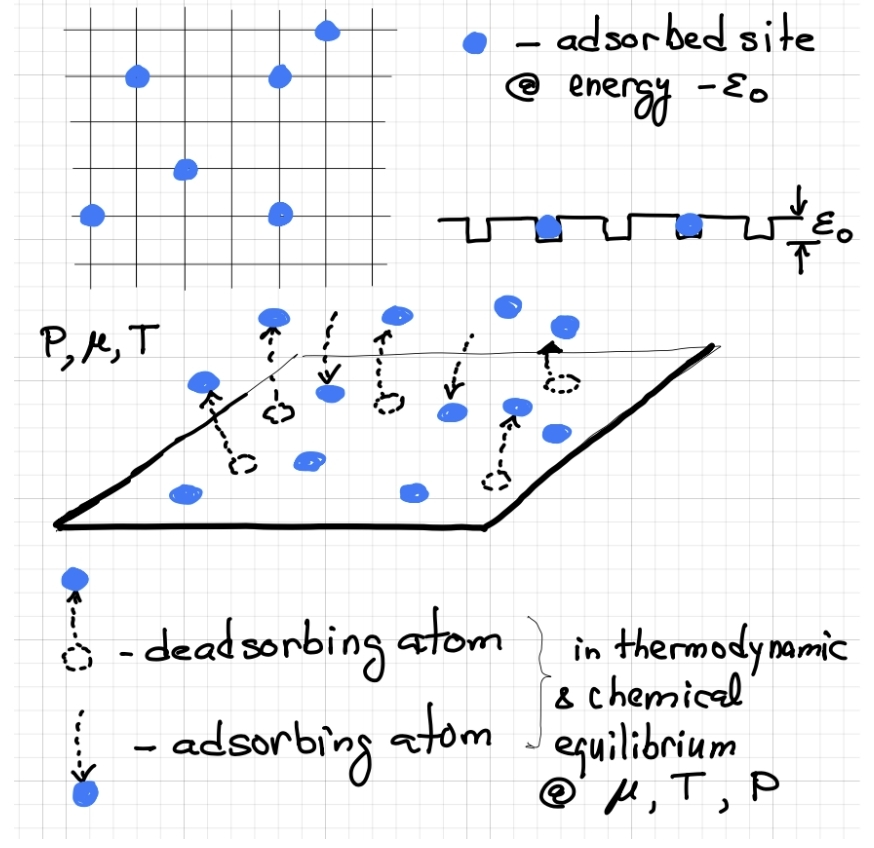
\includegraphics[width=0.6\textwidth]{hw3_p5.jpg}
    \caption{An illustration of a lattice gas with $N$ atoms occupying
    $N_0$ absorption sites at temperature $T$.}
    \label{fig:p5_illustration}
\end{figure}

\begin{enumerate}[label=(\alph*)]
    
\item ``Fermionic'' lattice gas

We first focus on the simplest case of only single maximum occupancy per site in
a single state of attractive energy $-\epsilon_0$. Thus, there are two states at
each site $0$ (unoccupied) and $-\epsilon_0$ (occupied by one atom), as
illutrated in \cref{fig:p5_illustration}.

\begin{enumerate}[label=(\roman*)]
    \item Compute the canonical partition function $Z(T,N)$, the corresponding
free energy $F(T,N)$, and calculate the corresponding chemical potential
$\overline{\mu}(T,N)$ as a function of prescribed fixed coverage
$N=\sum_{i=1}^{N_0}n_i$.
\begin{enumerate}[label=(\Alph*)]
    \item using $Z(T,N)$ from above, and 
    \item directly without going through $Z(T,N)$
\end{enumerate}

\begin{solution}
(A) First, note that with $N$ atoms to occupy $N_0$ sites, there are 
$\binom{N_0}{N}$ microstates with equal energy $\HH=-N\epsilon_0$. So the
canonical partition function is
\begin{equation}
    Z(T,N)=\binom{N_0}{N}\exp\qty(-\beta\HH)
    =\frac{N_0!}{N!(N_0-N)!}e^{N\epsilon_0/k_BT}.
\end{equation}
The free energy is thus
\begin{align}
    F(T,N)
    &=-k_BT\ln Z\notag\\
    &=-k_BT\qty[\frac{N\epsilon_0}{k_BT}+N_0\ln N_0-N\ln N-(N_0-N)\ln(N_0-N)].
\end{align}
Then it follows that the chemical potential is
\begin{equation}
    \overline\mu(T,N)
    =\frac{\partial F}{\partial N}
    =-\epsilon_0+k_BT\ln\qty(\frac{N}{N_0-N}).
\end{equation}

(B) By definition, the grandcanonical partition function is
\begin{equation}
    \ZZ=\qty[1+e^{\beta(\epsilon_0+\mu)}]^{N_0}.
\end{equation}
So the free energy is
\begin{equation}
    \FF=-N_0k_BT\ln\qty[1+e^{\beta(\epsilon_0+\mu)}],
\end{equation}
and the coverage is
\begin{equation}
    \overline{N}=-\frac{\partial\FF}{\partial\mu}
    =\frac{N_0}{1+e^{-\beta(\epsilon_0+\mu)}}.
\end{equation}
Inverting this expression, we get
\begin{equation}
    e^{-\beta(\epsilon_0+\mu)}=\frac{N_0-N}{N}
    \Rightarrow\mu=-\epsilon_0+\ln\qty(\frac{N}{N_0-N}),
\end{equation}
which agrees with result for $\overline\mu$ in part (A).

\end{solution}

\item Using $\ZZ(T,\mu)$ or $\FF(T,\mu)$ from either method above, compute the
    (1) entropy $S(T,\mu)$ and most importantly (2) the coverage -- the average
    number of particles $\overline{N}(T,\mu)$ and demonstrate that it agrees
    with the $\mu(T,N)$ expression obtained from the canonical ensemble.

\begin{solution}
In part (i-B), we have already calculated (2) the coverage and check the
agreement with $\overline\mu$ in (i-A). So now, using Mathematica, we 
calculate (1)
\begin{align}
    S(T,\mu)
    &=-\frac{\partial\FF}{\partial T}\notag\\
    &=N_0k_B\frac{\partial}{\partial
    T}\qty{T\ln\qty[1+\exp\qty(\frac{\epsilon_0+\mu}{k_BT})]}\notag\\
    &=N_0k_B\qty{\ln\qty[1+e^{(\epsilon_0+\mu)/k_BT}]-\frac{\epsilon_0+\mu}{k_BT}\frac{1}{1+e^{-(\epsilon_0+\mu)/k_BT}}}.
\end{align}
\end{solution}

\item Sketch $\overline{N}(T,\mu)$, discussing its low and high $T$ limits, and
    positive and negative $\mu$ limits. What is the characteristic value of the
    chemical potential $\mu$ at which the coverage changes at low $T$?
\begin{solution}
A contour plot is given below.
\begin{center}
    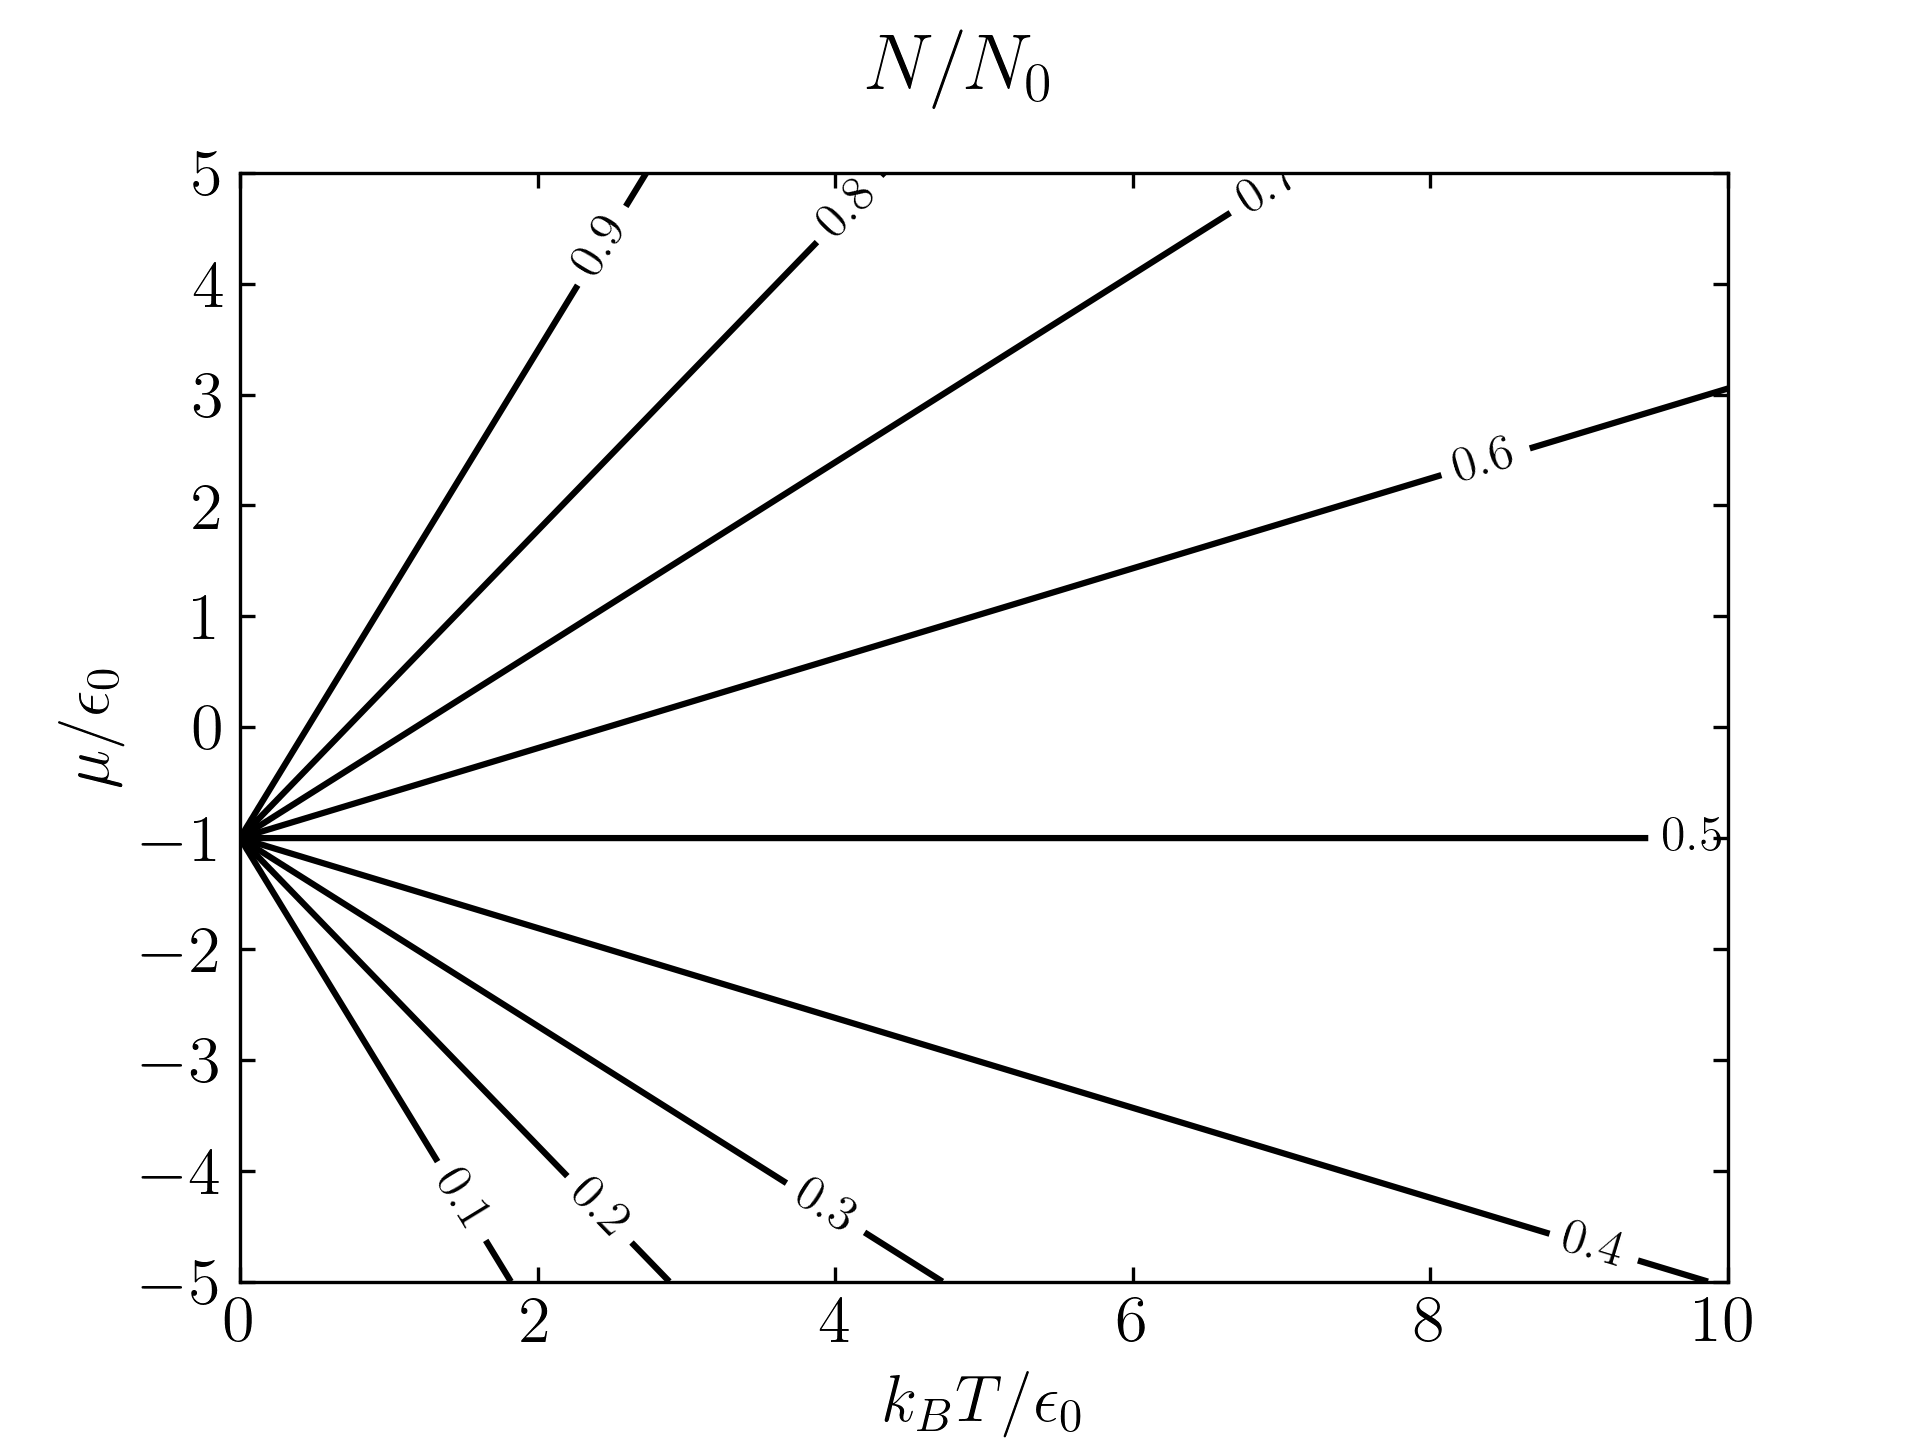
\includegraphics[width=0.7\textwidth]{p5a.png}
\end{center}
At low $T$ and negative $\mu$, there is almost no coverage as $N/N_0\to0$. At
low $T$ and positive $\mu$, $N/N_0\to1$ and the change occurs at
$\mu/\epsilon_0=-1$. At high $T$, the coverage changes less drastically for
negative and positive $\mu$.
\end{solution}

\item As discussed in class, the adsorbed atoms are in thermal and chemical
    equilibrium with the Boltzmann vapor above it, with a common temperature $T$
    and chemical potential $\mu$. Use this observation and your previous
    homework computation for the chemical potential of the Boltzmann gas to
    express your above result for coverage $\overline{N}(T,P)$ as a function of
    the pressure of the \textit{gas}.
\end{enumerate}
\begin{solution}
Because they are in chemical equilibrium, we can write the chemical potential
$\mu$ as
\begin{equation}
    \mu=k_BT\ln\qty(n\lambda_{dB}^3)
    =k_BT\ln\qty(\frac{P}{k_BT}\lambda_{dB}^3),
\end{equation}
where $\lambda_{dB}$ is the deBroglie wavelength and we have made use of the 
fact that a Boltzmann gas is ideal. Then, plugging
this into the expression for the coverage, we can write
\begin{equation}
    \overline{N}(T,P)=\frac{N_0}{1+(k_BT/P\lambda_{dB}^3)e^{-\epsilon_0/k_BT}}. 
\end{equation}
\end{solution}

\item ``Bosonic'' lattice gas

Now let's repeat the above analysis, but now allowing an arbitrary occupation of
sites, $n_i\in\qty{0,1,2,3,\hdots}$, and ignoring particle interactions, i.e.,
still having energy $-\epsilon_0$ per occupied particle.

\begin{enumerate}[label=(\roman*)]
    \item Calculate the grandcanonical partition function $\ZZ(T,\mu)$ and the
        corresponding free energy $\FF(T,\mu)$ for prescribed chemical potential
        $\mu$, directly, without going through $Z(T,N)$.

    \item Using $\ZZ(T,\mu)$ or $\FF(T,\mu)$ compute the (1) pressure
        $P(T,\mu)$, (2) entropy $S(T,\mu)$ and most importantly (3) the coverage
        -- the average number of particles $\overline{N}(T,\mu)$.

    \item Sketch $\overline{N}(T,\mu)$, discussing its low and high $T$ limits,
        and positive and negative $\mu$. Indicate unphysical regime of $\mu$ and
        speculate what actually happens in a physical system, namely what is the
        model missing to give physical answers.
\end{enumerate}
\end{enumerate}

\begin{solution}
(i) By definition and using the well-known geometric series
$\sum_{n\in\N}x^n=1/(1-x)$, we can calculate
\begin{equation}
    \ZZ=\qty[\sum_{n_i=0}^\infty e^{\beta(\epsilon_0+\mu)n_i}]^{N_0}
    =\qty[1-\exp\qty(\frac{\epsilon_0+\mu}{k_BT})]^{-N_0}.
\end{equation}
Then the free energy is
\begin{equation}
    \FF=-k_BT\ln\ZZ
    =N_0k_BT\ln\qty[1-\exp\qty(\frac{\epsilon_0+\mu}{k_BT})].
\end{equation}

(ii) Then it folows that (1) the pressure is
\begin{equation}
    P(T,\mu)=-\frac{\partial\FF}{\partial V}=0,
\end{equation}
(2) the entropy is
\begin{equation}
    S(T,\mu)
    =-\frac{\partial\FF}{\partial T}
    =N_0k_B\qty[\frac{\epsilon_0+\mu}{k_BT}\frac1{1-\exp\qty[-(\epsilon_0+\mu)/k_BT]}-\ln\qty[1-e^{(\epsilon_0+\mu)/k_BT}]],
\end{equation}
(3) the coverage is
\begin{equation}
    \overline{N}
    =-\frac{\partial\FF}{\partial\mu}
    =\frac{N_0}{1-\exp\qty[-(\epsilon_0+\mu)/k_BT]}.
\end{equation}

(iii) A plot of $\overline{N}$ is included below.
\begin{center}
    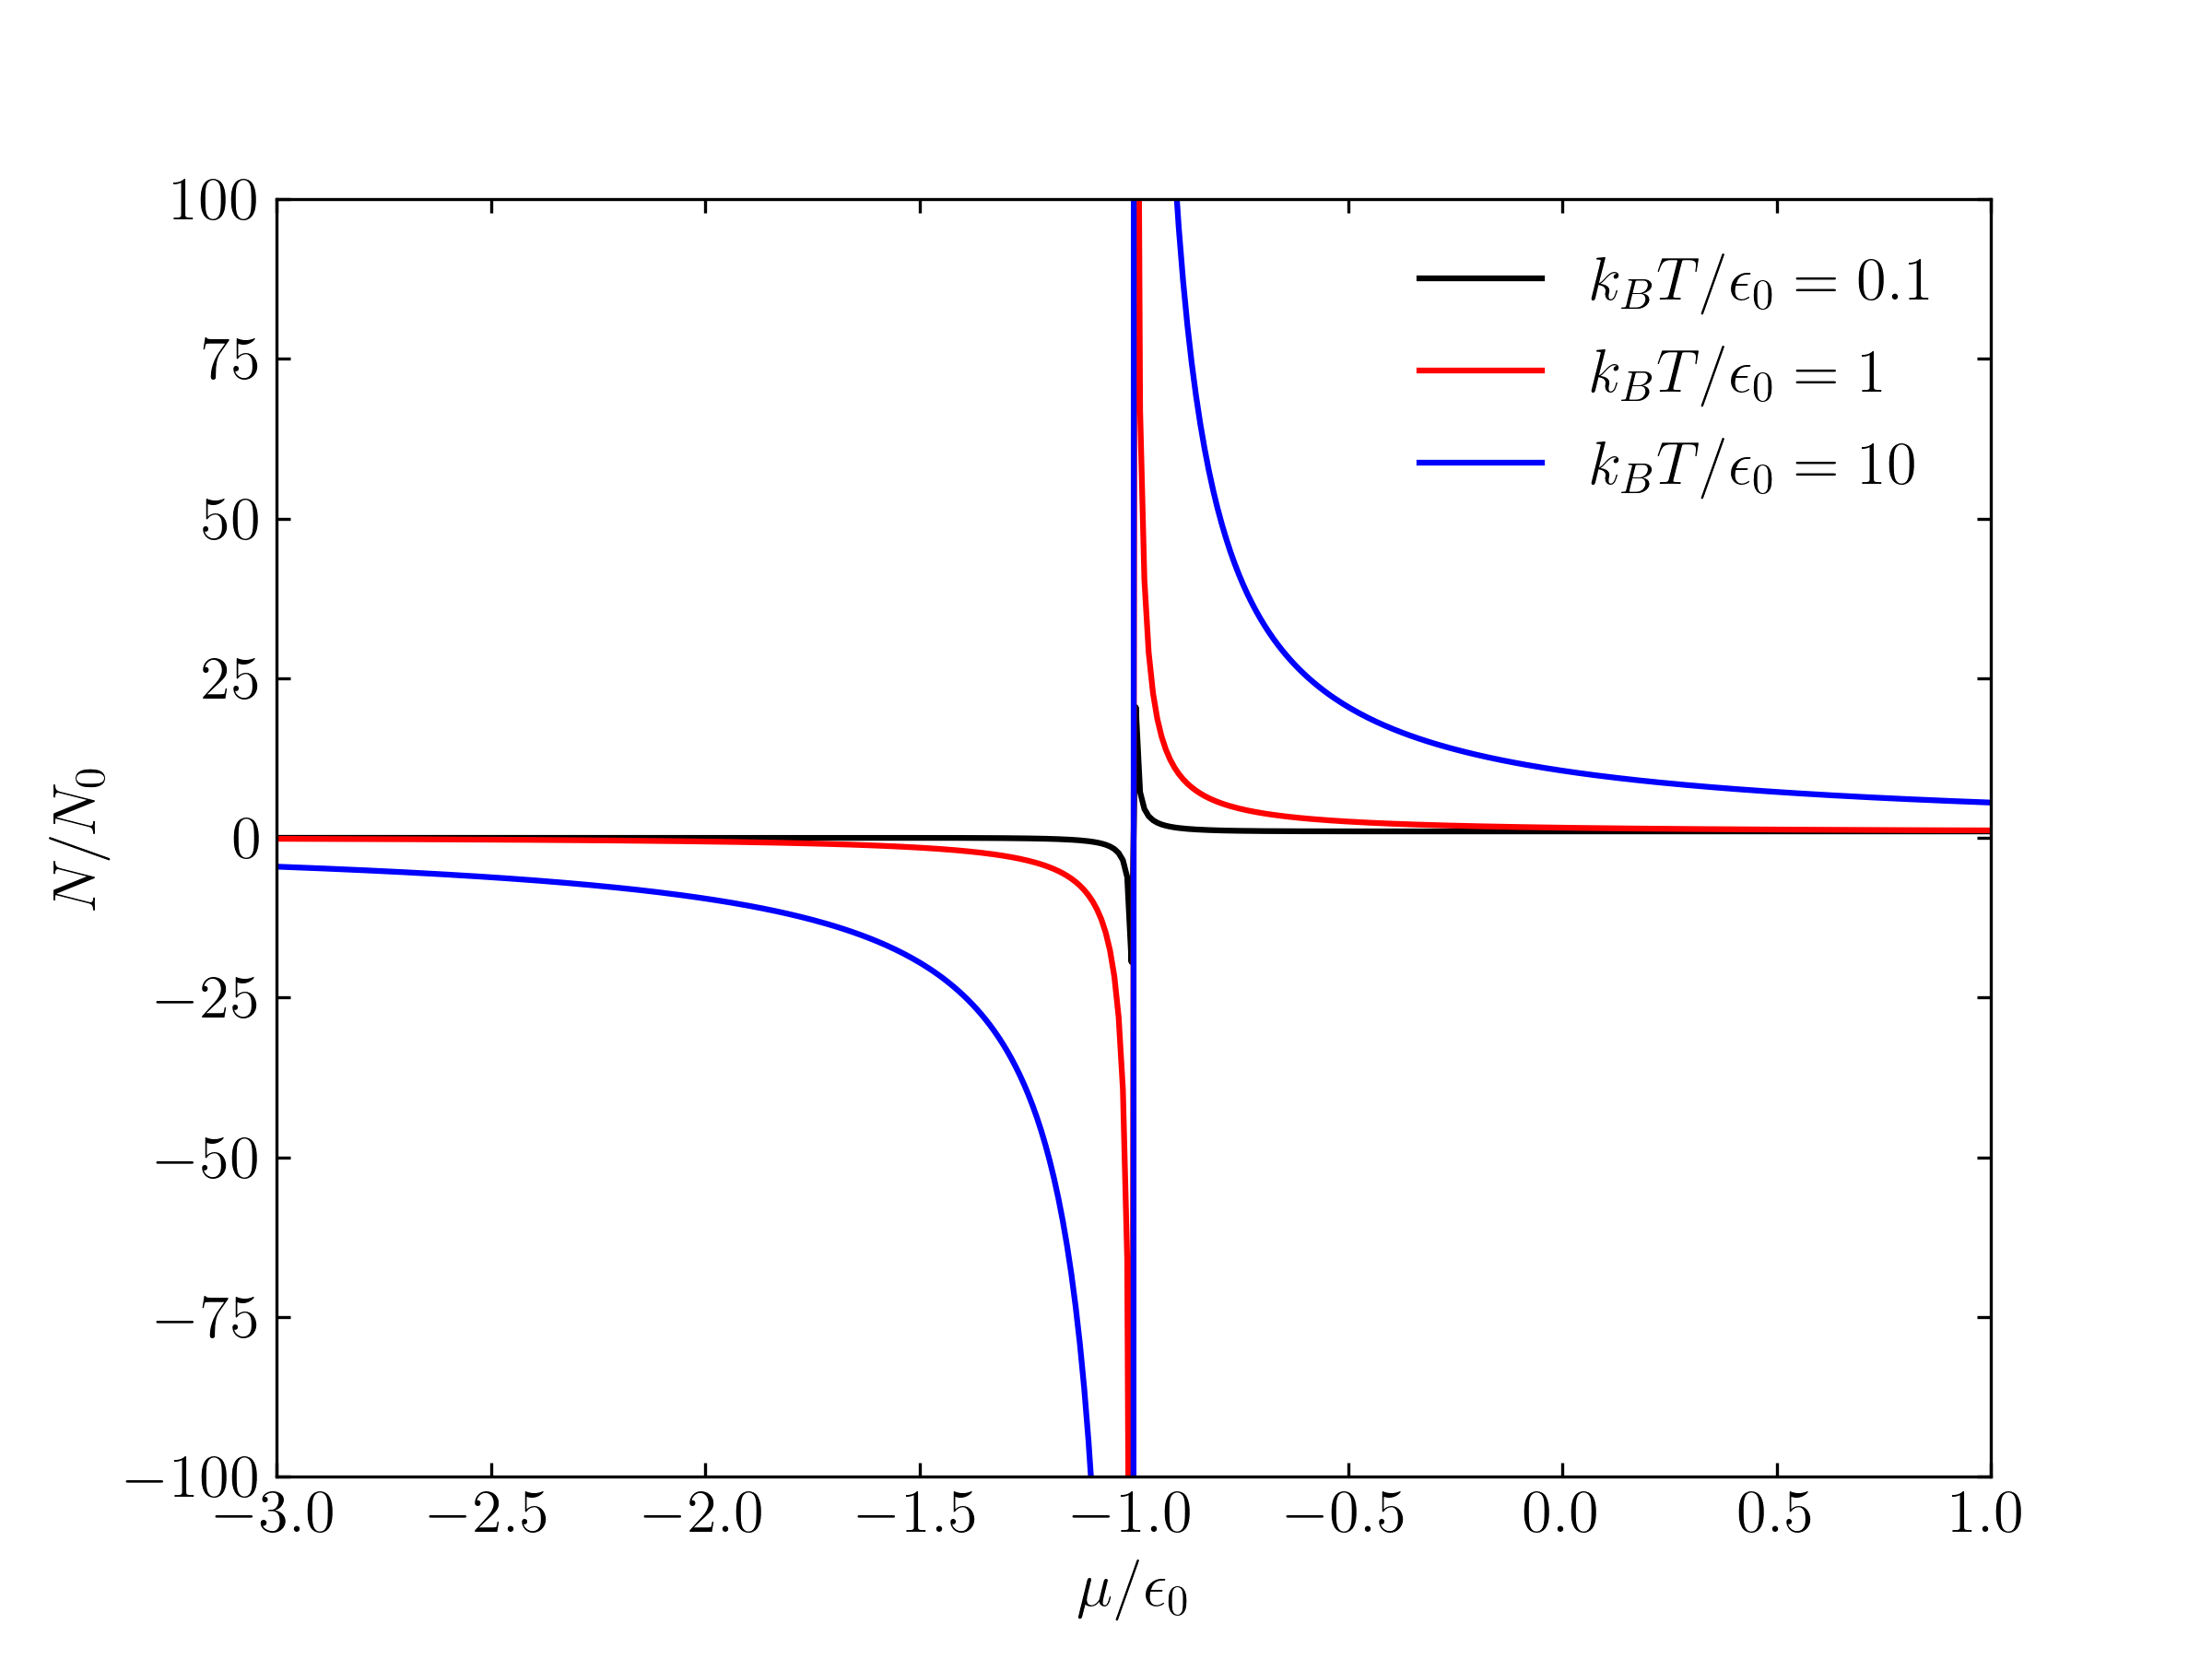
\includegraphics[width=0.7\textwidth]{p5b.png} 
\end{center}
The behavior is very different from the Fermionic case. Both at low and high
$T$, the coverage vanishes everywhere except for when $\mu=-\epsilon_0$. At
negative and positive $\mu$, $\overline{N}$ also vanishes. Clearly, $N$ cannot
be negative, so the unphysical range of $\mu$ is $\mu\leq-1$. This model, since
it allows for infinite occupation, can intuitively lead to $\overline{N}$
blowing up. By restricting the maximum occupation for each site, it should 
give a more physical answer.
\end{solution}
\end{problem}
\newpage
%%%%%%%%%%%%%%%%%%%%%%%%%%%%%%%%%%%%%%%%%%%%%%%%%%%%%%%%%%%%%%%%%%%%%%%%%%%%%%%
\end{document}
